% !TeX root = ./main.tex
\documentclass[11pt,oneside]{book}

\usepackage[utf8]{inputenc}
\usepackage[english, danish]{babel}
\usepackage{datetime}  

\usepackage[margin=1.2in]{geometry}
\usepackage[toc,page]{appendix}
\usepackage{graphicx}
\usepackage{natbib}
\usepackage{lipsum}
\usepackage{caption}
\usepackage{subcaption}
\usepackage[hidelinks]{hyperref}
\usepackage{tikz}
\usepackage{array}
\usepackage{float}

\usetikzlibrary{shapes,arrows}
\usetikzlibrary{positioning}

\makeatletter
\renewcommand{\@makechapterhead}[1]{%
   {\parindent \z@ \raggedright \normalfont
     %\ifnum \c@secnumdepth >\m@ne
     %    \huge\bfseries \@chapapp\space \thechapter
     %    \par\nobreak
     %    \vskip 20\p@
     %\fi
     %\interlinepenalty\@M
     \Huge \bfseries\thechapter\space\space #1\par\nobreak
     \vskip 30\p@
   }}
\makeatother


% Rename appendix to bilag
\renewcommand\appendixname{Bilag}
\renewcommand\appendixpagename{Bilag}
\renewcommand\appendixtocname{Bilag}


% Remove indentation
\setlength\parindent{0pt}

% Define a command  for citing in a footnote
\newcommand*{\footcite}[1]{\footnote{\cite{#1}}}

\newdimen\zerolinewidth

\tikzset{
  zero line width/.code={%
    \zerolinewidth=\pgflinewidth
    \tikzset{line width=0cm}%
  },
  use line width/.code={%
    \tikzset{line width=\the\zerolinewidth}%
  },
  draw with anchor in boundary/.style={
    zero line width,
    postaction={draw,use line width},
  },
}

\newcolumntype{L}[1]{>{\raggedright\let\newline\\\arraybackslash\hspace{0pt}}m{#1}}
\newcolumntype{C}[1]{>{\centering\let\newline\\\arraybackslash\hspace{0pt}}m{#1}}
\newcolumntype{R}[1]{>{\raggedleft\let\newline\\\arraybackslash\hspace{0pt}}m{#1}}


\begin{document}

%\captionsetup[figure]{margin=1.5cm,font=small,labelfont={bf},name={Figure},labelsep=colon,textfont={it}}
%\captionsetup[table]{margin=1.5cm,font=small,labelfont={bf},name={Table},labelsep=colon,textfont={it}}
\SetLipsumDefault{1}

\frontmatter

% === Titlepage ===
\begin{titlepage} 
    \begin{center}
        {\LARGE IT University of Copenhagen}\\[1.5cm]
        \linespread{1.2}\huge {\bfseries saWux Visualizer}\\
        \linespread{1.2}\large {\bfseries Gruppe 16, Projektrapport}\\[1.5cm] % Ændr til samarbejdsrapport
        \linespread{1}
        
\includegraphics[width=5cm]{Images/logo.png}\\[1cm]  % Billede af løsningen
        {\large
        \begin{tabular}{R{0.465\textwidth}  L{0.465\textwidth}}
            Albert Rise Nielsen & albn@itu.dk\\
            Alyson De Souza 	& ades@itu.dk\\
            Joachim Kofoed 	    & jkof@itu.dk\\
            Markus Johansen 	& mkjo@itu.dk\\
            Peter Fuchs 	    & pefu@itu.dk\\
            Simon Johann Skødt	& sijs@itu.dk\\
            Simon W. Gundersen 	& sgun@itu.dk\\
            Victor Brorson 	    & vibr@itu.dk
        \end{tabular}}\\[1cm]

        {\large \emph{Kursus:} Projektarbejde og Kommunikation 2020}\\
        {\large \emph{Kursuskode:} BSPRKOM1KU}\\[1cm]
        \today
    \end{center}        
\end{titlepage}



% === Table of contents, figures and tables ===
\tableofcontents
\listoffigures
%\listoftables


% === Main ===
\mainmatter

\chapter{Indledning}
\section{Baggrund for rapport}
Denne rapport er skrevet i forbindelse med projektarbejdeforløbet i faget \emph{Projektarbejde og Kommunikation} på 1. semester af bacheloruddannelsen Softwareudvikling på IT-Universitetet i København. Rapporten er udarbejdet med henblik på at løse et problem, givet af virksomheden \emph{SC-Tronics} (SC-T) i forbindelse med lancering af deres nye produkt \emph{saWux}. Udfordringen går på at forbedre datavisualiseringen for \emph{saWux'} produkter, således at den viste data skaber mest mulig værdi for kunden.\\
Rapporten danner grundlag for at assistere virksomheden i at omstrukturere deres allerede eksisterende app med henblik på bedre visualisering af data.

\section{Problemfelt}
Flere virksomheder og husstande ønsker øget kontrol og forståelse for deres energiforbrug \citep{klimaindsats} — for både at spare penge og blive mere bæredygtige. Statistiske og grafiske værktøjer er fordelagtige i forbindelse med at øge netop kontrollen, og de skaber et bedre overblik for brugerne af deres energiforbrug \citep{herrmann}. I store virksomheder anvendes allerede omfattende værktøjer, komplekse løsninger og store pengesummer til at optimere energiforbruget. Ifølge det danske udviklings- og energistyringsfirma SC-T eksisterer der et hul i markedet for løsninger til private husstande og til de små og mellemstore virksomheder \citep{sawux}.

\section{Problemstilling}
SC-Tronics har udarbejdet løsningen \emph{saWux} til energistyring og dataindsamling, som iværksættervirksomheden i skrivende stund lancerer i de kommende måneder. En udfordring er, at data ikke fremstår tydeligt for brugeren af den tilknyttede \emph{saWux}-app. Observation og visualisering af data spiller en central rolle i, at målgruppen har lyst til at investere i og bruge SC-T produkter. Når kunden investerer i \emph{saWux}, regner man med besparelse på 10-20 procent i energiforbrug om året \citep{sawux}, hvilket skal gøres klart og forståeligt for brugeren. Appen muliggør at kontinuerligt observere elforbruget, men kommunikationen og formidling af eventuelle besparelser og data fra virksomhedens øvrige enheder er enten ikke tilstedeværende eller uklart.

\section{Problemformulering}
Hvordan kommunikerer og visualiserer SC-T elforbrug til de private husstande med særligt henblik på familier med hjemmeboende børn, således at målgruppen motiveres til strømbesparende adfærd og aktiv, miljørigtig handling?            \newpage
\chapter{Problemanalyse}
\section{Identifikation af problem}
SC-Tronics præsenterer sin nye IoT-løsning \emph{saWux} til en fremlæggelse på ITU, d. 24-08-2020. \emph{saWux} er en datadrevet energi- og klimastyringsløsning, der har til formål at udskifte den konventionelle stikkontakt med alt fra automatiserede stikkontakter og watt-målere til stikkontakter med timere, CO$_2$-målere, temperaturmåling og luftkvalitetsmåling \citep{sawux}.\\

I den sammenhæng stiller SC-T udfordringen, at de søger hjælp til at visualisere den data, som \emph{saWux} indsamler, således at det giver mening og overskueliggøres for deres brugere \citep{virksomhedspresentation}. Problemstillingen er dels at finde en målgruppe og få indsigt i denne — til fordel for både SC-T i fremtiden og ikke mindst for projektet. Desuden beder SC-T om hjælp til den kreative proces, for at skabe den bedste visualisering som muligt og skabe nye idéer til, hvordan man effektivt illustrerer en større mængde data \citep{virksomhedspresentation}.\\

\section{Fremgangsmåde og metoder}
Den første research undersøger, hvordan man effektivt visualiserer data, samt om der eksiterer andre produkter og konkurrenter på markedet, der udbyder det samme som \emph{saWux}. Ved læsning og research af empiri og artikler blev der dannet et grundlag for udarbejdelsen af egen visualisering, som skal eksemplificeres ved hjælp af en mockup og en teknisk beskrivelse.\\

Herefter defineres en målgruppe, som det giver mening at appellere til. Familier med hjemmeboende børn kommer hurtigt på tegnebrættet på baggrund af interesse og tilgængelighed. Under et interview med SC-T gør de selv udtryk for interesse i denne målgruppe.\\

Teorien og empirien udbygges nu på baggrund af målgruppen. En brugerundersøgelse udarbejdes (se bilag \ref{appendix:survey}), som påpeger, at Line Charts — hvor hvert punkt på grafen aflæses med markøren — er et godt grafværktøj til at sammenligne data. Derudover viste undersøgelsen, at der er en indikator, der beskriver den gennemsnitlige værdi ved siden af hver graf (bilag \ref{appendix:survey}). Metoderne, der er blevet brugt, er altså en blanding mellem kilde- og dataresearch samt indsamling af egen data i form af både kvantitative og kvalitative undersøgelser.\\

\section{Målgruppeanalyse}
\cite{osterwalder} fremhæver i teori for “Value Proposition Design”, hvordan virksomheders produkter skal tiltænkes kunden. På den ene side undersøges kundernes profil, mens produktet på den anden side sættes i højsædet, hvilket skaber værdi for kunden.\\

Målgruppen for vores løsning er familier med hjemmeboende børn, med henblik på især at ramme familiens overhoved. Denne målgruppe er interessant, fordi interessen for at spare på kWh-forbruget i husstande stiger \cite[p. 34]{ens.dk}. Familier med hjemmeboende børn er særligt attraktive, da der er tale om et generationsmøde, hvoraf den yngre generation er stærkt klimabevidste \citep{energiwatch}. Flere studier — som for eksempel \cite{gronhoj} — peger på at forældrenes klimahandlinger smitter af på deres børn, og dermed er flere forældre opsatte på at være eksemplariske. \emph{saWux} tilbyder løsningen, der stiller det gode eksempel — og tilmed muliggør \emph{saWux Visualizer}-appen inddragelse af hele familien.

\subsection{Kvantitativt brugerundersøgelse}
I forbindelse med udarbejdelsen af vores visualiseringsapplikation, konstruerer vi en undersøgelse med henblik på at finde den mest brugervenlige visualiseringsværktøj (se bilag \ref{appendix:survey}). Vi når ud til 38 mennesker i alderen 0 til 60. Visualiseringsmetoderne bliver vurderet og rangeret i et pointsystem, der ligger til grundlag for de valgte grafer og udseender i \emph{saWux Visualizer}.

\subsection{Kvalitativt interview}
I forbindelse med udarbejdelsen af vores \emph{Value Proposition Canvas} interviewes et individ fra vores målgruppe (se bilag \ref{appendix:interview}). Interviewet har til formål at opnå en højere indsigt af kundernes “Customer Profile”. Resultatet af interviewet be- og afkræfter flere af de forventninger, der er til kundens jobs, pains og gains. Hermed illustreres kundernes behov gennem “The Value Proposition Canvas” \citep{osterwalder}, hvorfor SC-T’s målgruppe udspecificeres. Illustreret nedenfor i figur \ref{img:problem:canvas}.

\begin{figure}[H]
    \centering
    \includegraphics[width=0.5\textwidth]{Images/Value Proposition Design.png}
    \caption[\emph{Value Proposition Canvas}]{\emph{Value Proposition Canvas}, der viser brugerens \emph{jobs, pains} og \emph{gains}}
    \label{img:problem:canvas}
\end{figure}

\section{Resultater til beslutninger}
SC-Tronics fortæller til præsentationen på ITU — og skriver det desuden på \emph{saWux} egen hjemmeside — at de har flere målgrupper, de gerne appellerer til med sit produkt (\cite{virksomhedspresentation} og \cite{sawux}).
Til dels målretter de sig til både private og offentlige virksomheder, og dels til de private forbrugere og “DIY handymen- og girls” \cite{sawux}. SC-Tronics profilerer \emph{saWux} på at være let tilgængelig, billig, intuitiv og mulig at installere selv — uden en autoriseret el-installatør \citep{virksomhedspresentation}. Det er de private forbrugere, dette projekt fokuserer på; det er målgruppen til visualiseringen af \emph{saWux}' data. Mere konkret; familier med hjemmeboende børn. Dette valg er taget for at kunne ramme samspillet mellem to generationer — de energitænkende og  miljøbevidste \citep{energiwatch}. Allerede IT-kompetente og miljøbevidste forældre vil gerne forbedre sine børns liv og give bevidstheden videre til deres børn. \citep{stacey}.\\

Resultatet af de to undersøgelser viser, at denne målgruppe står med et ønske om at spare penge og få et bedre overblik over sit forbrug i en travl hverdag. Målgruppen har en god forståelse af simple grafer med interaktivitet og gennemsnitlige tal (se bilag \ref{appendix:survey}).        \newpage
\chapter{Teknisk beskrivelse}
I det følgende kapitel beskrives applikationen \emph{saWux Vizualizer}. Her lægges der vægt på forklare de relevante delkomponenter.

\section{Teknisk definition}
Inden for datavisualisering er \emph{saWux Vizualizer} en visualiseringsapplikation, der illustrerer data fra \emph{saWux} enheder i husstande med hjemmeboende børn. \emph{saWux Vizualizer} indhenter henholdsvis kWh, CO$_2$, forbrug i kroner og tænde-/slukketid i de pågældende husstande, og illustrerer dette på en simpel og forståelig måde. Desuden tilbyder appen et konkurrence- og spil element, således at familier kan dyste i at opnå den højeste besparing.

\section{Løsningens delkomponenter}
\emph{saWux Vizualizer} består af flere delelementer, hvoraf de vigtigste er beskrevet i dette afsnit: \emph{Infrastruktur}, \emph{Dashboard}, \emph{Cards}, \emph{Family Mode} og \emph{Inspiration Mode}. 

\subsection{Infrastruktur}
% TODO: Fix this
\begin{figure}[H]
    \centering
    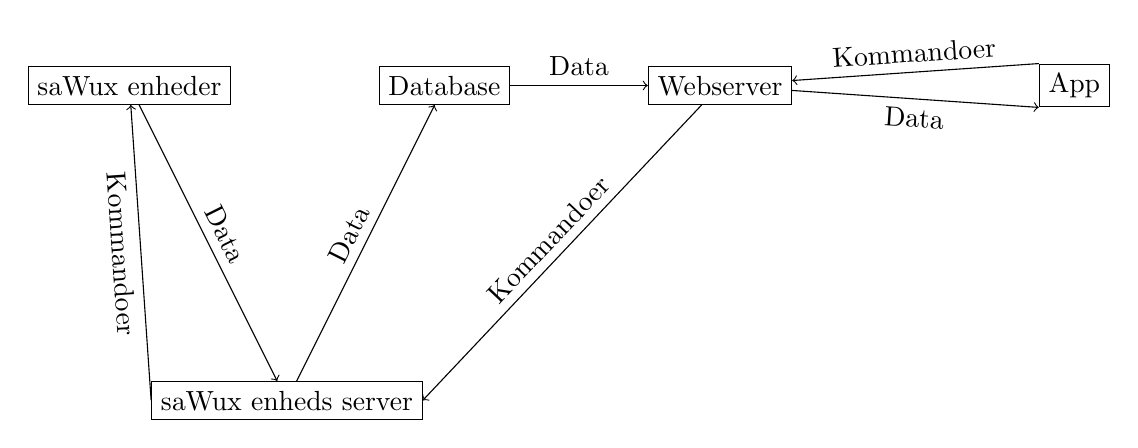
\begin{tikzpicture}
        \node at (0,0) [rectangle,draw] (devices) {saWux enheder};
        \node at (2,-4) [rectangle,draw] (deviceServer) {saWux enheds server};
        \node at (4,0) [rectangle,draw] (database) {Database};
        \node at (7.5,0) [rectangle,draw] (webserver) {Webserver};
        \node at (12,0) [rectangle,draw] (app) {App};

        \draw[->] (deviceServer.west) -- (devices) node [midway, below, sloped] {Kommandoer};
        \draw[->] (webserver)    -- (deviceServer.east) node [midway, above, sloped] {Kommandoer};
        \draw[->] (app.north west)          -- (webserver) node [midway, above, sloped] {Kommandoer};

        \draw[->] (devices)      -- (deviceServer) node [midway, above, sloped] {Data};
        \draw[->] (deviceServer) -- (database) node [midway, above, sloped] {Data};
        \draw[->] (database)     -- (webserver) node [midway, above, sloped] {Data};
        \draw[->] (webserver)    -- (app.south west) node [midway, below, sloped] {Data};
    \end{tikzpicture}
    \caption[Diagram over infrastruktur]{Diagram over \emph{saWux Visualizers} infrastruktur}
    \label{img:teknisk:infra}
\end{figure}
Løsningens infrastruktur, der ses i figur \ref{img:teknisk:infra}, består af en række af elementer. Det første element er sensorer og enheder, leveret af \emph{saWux}. Disse kan modtage kommandoer såsom tænd og sluk fra enhedsserveren. Enhederne sender ligeledes sensordata; blandt andet information om sig selv til enhedsserveren. Enhedsserveren gemmer den modtagne data i en database. Til databasen hører en webserver, der kan sende dataen videre til en app, når appen beder om det. Webserveren kan også modtage kommandoer fra appen og videresender dem til enhedsserveren, som videresender dem til enhederne, der udfører kommandoen. Det sidste element er appen.\\ 

Appen er ansvarlig for at vise enhederne og dataen grafisk, så det er forståeligt for brugeren. Appen er også brugerens måde at interagere med enhederne — ved at lade dem sende kommandoer, såsom tænd og sluk ved at trykke på en knap.

\subsection{Dashboard}
Inden for \emph{saWux Visualizer} er \emph{Dashbordet} er applikationens start- og hovedside. Et interface — hvis hovedformål er at give et generelt overblik over husstandens forbrug. Fra \emph{dashboardet} kan brugeren tilgå alle applikationen delelementer, som er beskrevet nedenfor. Forbruget bliver vist i form af forskellige \emph{cards}, brugerne selv kan tilføje, slette og rykke rundt på. 
\begin{figure}[H]
    \centering
    \includegraphics[width=\textwidth]{Images/Main Board.png}
    \caption[\emph{Dashboard} mockup]{Mockup af \emph{saWux Visualizers dashboard}}
    \label{img:teknisk:dashboard}
\end{figure}

\subsection{Cards}
Inden for \emph{saWux Visualizer} er \emph{cards} applikationens visuelle fremstillingsmetode. Formålet med hvert \emph{card} er, at fremstille den indsamlede data på den mest brugervenlige måde. Dette gøres i form af et interaktivt element, der giver brugeren muligheden for at designe hvert \emph{card}, således at det giver den mest optimale individuelle forståelse. Card tilføjes ved at trykke på \emph{+ ikonet} (se figur \ref{img:teknisk:addcard}). Ved tilføjelsen af et \emph{card} gennemløber brugeren en udvælgelsesproces af følgende elementer:
\begin{itemize}
    \item Cardtype — Formålet med dette \emph {card}.
    \item Datatype — Hvilken dataype skal det givne \emph {card} vise.
    \item Graftype — Hvilke graftype skal det givne \emph {card} vise.
    \item Room — Hvilket rum skal det givne \emph {card} indhente data fra.
\end{itemize}
\begin{figure}[H]
    \centering
    \includegraphics[width=\textwidth]{Images/Add Card.png}
    \caption[Tilføj \emph{card} mockup]{Mockup af funktionen der tilføjer \emph{cards} i appen}
    \label{img:teknisk:addcard}
\end{figure}
På figur \ref{img:teknisk:card} nedenfor ses et eksempel på et \emph{card}, der viser forbruget i \emph{living room}. Dette \emph{card} er opbygget med en interaktiv line-graph, hvor interval af tid findes på $x$-aksen og forbrug af kWh på $y$-aksen. Flytter brugeren på forstørrelsesglas-ikonet, er outputtet det specifikke tal på den givne tid. Desuden illustreres gennemsnitsforbruget for det valgte tidsinterval (D/U/M/Å).
\begin{figure}[H]
    \centering
    \includegraphics[width=\textwidth]{Images/Main Board - Card.png}
    \caption[\emph{Card} mockup]{Mockup af et specifikt \emph{card}, der viser forbrug af kWh}
    \label{img:teknisk:card}
\end{figure}
\newpage

\subsection{Family Mode}
Inden for \emph{saWux Visualizer} er \emph{Family Mode} et interface, hvor husstanden kan konkurrere i at have den største besparelse. Dette gøres via en spilfunktion, hvor familien kan sammenligne forskellige forbruget i forskellige rum (børneværelset, stuen, ect.). Ved at trykke på \emph{controller +} ikonet øverst i venstre hjørne, får brugeren mulighed for at tilføje forskellige spil og dertil deltagere. Herfra kan familien eksempelvis konkurrere i at bruge færrest kWh, og samtidig se hvem, der klarer sig bedst. Trykker brugeren på \emph{podie-ikonet} øverst til højre, bliver hele historikken af sejre — tidsperioden definerer brugeren selv — visualiseret.
\begin{figure}[H]
    \centering
    \includegraphics[width=0.8\textwidth]{Images/Kids mode.png}
    \caption[\emph{Family Mode} mockup]{Mockup af funktionen \emph{Family Mode}}
    \label{img:teknisk:kidsmode}
\end{figure}

\subsection{Inspiration Mode}
Inden for \emph{saWux Visualizer} er \emph{Inspiration Mode} applikationens \emph{news feed interface}, hvor brugeren kan tilgå de nyeste informationer om \emph{saWux'} publikationer. Dette interface viser de tre nyeste publiceringer, som illustreres med et \emph{card}, der viser en kategori, en overskrift og et billede. Trykker brugeren på et af de tre \emph{cards}, folder artiklen sig ud og brugeren læser sig til en bedre forståelse af forbrug (el, gasser, etc.), tips og tricks til besparelse samt nye produkter og så videre.
\begin{figure}[H]
    \centering
    \includegraphics[width=\textwidth]{Images/Open An Article.png}
    \caption[\emph{Inspiration Mode} mockup]{Mockup af \emph{Inspiration Mode}, der viser artikler om blandt andet miljø- og forbrugsbesparelser}
    \label{img:teknisk:article}
\end{figure}
\subsection{Transitions}
Inden for \emph{saWux Visualizer} er \emph{Transitions} måden hvorpå brugeren bevæger sig rundt i applikationen. Overgangen mellem \emph{dashboardet} og applikationens andre interfaces (\emph{Family Mode} og \emph{Inspiration Mode}) sker gennem \emph {navigationsboardet}, som er den menu, der ses nederst på \emph{dashboardet}. Når eksemplevis \emph {Family Mode} er valgt, folder en hvid lokal \emph{bar} med nye funktioner sig ud i toppen af skærmen, således at man kan tilgå og bruge lokale funktioner i den valgte \emph{Mode}. Den miderste knap med en opadvendt pil har samme funktion i alle lokale \emph{Modes}. Funktionen sender brugeren tilbage til \emph {dashboardet}, hvorfra man igen kan tilgå de andre \emph {Modes}.
\begin{figure}[H]
    \centering
    \includegraphics[width=0.9\textwidth]{Images/Transitions.png}
    \caption[\emph{Transitions} mockup]{Mockup af \emph{transitions} eller \emph{overgange} mellem appens forskellig funktioner og sider}
    \label{mockupg:teknisk:transitions}
\end{figure}

\section{Opsummering}
\emph{saWux Visualizer} indsamler data fra \emph{saWux} enheder og giver hurtigt brugeren et overblik over husstandens forbrug. Applikationen er opbygget af interaktive interfaces, der hovedsageligt designes af brugerne selv ved hjælp af forskellige \emph{cards}. Samspillet mellem \emph{saWux Visualizers} delelementer giver brugeren et hurtigt overblik over sine besparelser. Desuden muliggør applikationen at familier kan konkurrere mod hinanden og få inspiration til nye besparelsesmetoder eller andre \emph{saWux} produkter. 
   \newpage
\chapter{Brugerscenarie}
For at uddybe funktionaliteten af vores produkt opstilles et brugerscenarie, der inddrager en far og hans datter.\\

\textbf{Bruger 1:}\\
\textbf{Navn:} Karsten\\
\textbf{Køn og Alder:} Mand, 45 år\\
\textbf{Rolle:} Familiefar og tech-entusiast\\
\textbf{Brug:} Skabe overblik og kontrol over energiforbruget i forskellige dele af huset\\[0.5ex]

\textbf{Bruger 2:}\\
\textbf{Navn:} Lotte\\
\textbf{Køn og Alder:} Pige, 13 år\\
\textbf{Rolle:} Datter til Karsten; går i 5. klasse\\
\textbf{Brug:} Konkurrence mellem familiemedlemmer\\[0.5ex]

\begin{enumerate}
    \item Karsten kommer hjem fra arbejde og åbner \emph{saWux Visualizer} på sin smartphone.
    \item Han scroller igennem sit \emph{dashboard} og ser, at der er blevet brugt usædvanligt meget strøm i huset i løbet af dagen.
    \item Karsten undersøger problemet og opdager hurtigt, at fjernsynet har stået tændt, uden at nogen brugte det. 
    \item For at få bedre overblik over strømforbruget fra fjernsynet opretter han et nyt \emph{card} på sit \emph{dashboard}, der ser strømforbruget i stuen, hvor fjernsynet befinder sig. Karsten vælger at visualisere strømforburget via en graf.

    \item Lotte kommer hjem fra skole og sætter sig på sit værelse, hvor hun tænder for sit fjernsyn.
    \item Hun åbner \emph{saWux Visualizer}, der allerede er inde på \emph{Family Mode}. Her kan hun se familiens igangværende \emph{First to 25}-konkurrence. Hun observerer under \emph{Rankings}, at hun har brugt flest kWh og derfor er ved at tabe konkurrencen. 
    \item Hun beslutter sig for at slukke for fjernsynet, stikkontakten ligeledes, for at spare på strømmen.
    \item Lotte ser på sit \emph{dashboard}, at dette får strømforbruget på hendes værelse til at falde.
    \item Samtidig sidder Karsten i familiens stue og scroller igennem \emph{Inspiration Mode} i \emph{saWux Visualizer}.
    \item Her opdager han en artikel med gode råd til hans \emph{saWux} produkter.
\end{enumerate}

        \newpage
\chapter{Test}
Dette afsnit giver et overordnet forslag til, hvilke metoder der er relevante ved udførelsen af en teknisk test samt en brugertest af \emph{saWux Visualizers} delelementer og opstiller succeskriterierne for denne test \cite[Kap. 9]{finkelstein}.

\section{Teknisk test}
\emph{saWux Visualizer} er en moderne og fleksibel brugergrænseflade, der kombineres med en stor mængde af data. Fejl i præsentationen af data har store konsekvenser for \emph{SC-Tronics} troværdighed.

\subsection{Fremgangsmåde}
Back-end developers anvender tekniske unit tests til at sikre det korrekte dataflow, som beskrevet i figur \ref{img:teknisk:infra}.

\subsection{Succeskriterie}
De tekniske tests skal sørge for at:
\begin{itemize}
    \item Forbindelsen mellem app og produkt er optimal og fejlfri.
    \item Kundens anmodede oplysninger matcher output-data og dens tilsvarende grafer med pålidelig information.
    \item Kunden navigerer gnidningsfrit gennem de forskellige \emph{dashboards} og \emph{cards}.
\end{itemize}

\section{Brugertest}
Gruppens tilgang til bedre datavisualisering af kundens data er baseret på forskellige delelementer: \emph{Dashboard, Cards, Family Mode, Inspiration Mode} og \emph{Inspiration}, der giver kunden et bedre overblik over sit energiforbrug og motiverer denne til at tage en aktiv handling i retning mod dette formål.

\subsection{Fremgangsmåde}
Udvikling af en dummy-app kan skabe et indblik i, om appen opfylder målene opstillet i Value Proposition Canvas (Figur \ref{img:problem:canvas}).

\subsection{Succeskriterie}
\emph{saWux Visualizers} dummy-app til indsamling af data påviser, at:
\begin{itemize}
    \item Målgruppen forstår grafer ved aktiv handling til at opnå en økonomisk besparelse i forhold til sit førhenværende energiforbrug.
    \item Anvendelse af \emph{saWux Visualizer — First to 25}-konkurrencen engagerer hele familien til aktiv, energibesparende handling.
    \item Brug af \emph{saWux Visualizer — Inspiration Mode} bekræfter, hvorvidt der findes interesse i henholdsvis økonomisk besparelse samt en stigende bevidsthed om indeklima og miljø.
\end{itemize}


                  \newpage
\chapter{Konklusion}
I arbejdet med problemformuleringen udvikles et mock-up af applikationen \emph{saWux Visualizer}. Et simpelt og interaktivt visualiseringsverktøj, der gør data fra \emph{saWux} forståelig og let tilgængelig for hele hustanden. \emph{saWux Visualizer} indeholder den såkaldte \emph{Family Mode}, for hvilket den opfordrer til inddragelse af hele familien. Kombinationen af disse elemeter synes at fremme strømbesparende adfærd, klimabevidste handlinger og dermed en økonomisk gevinst.\\

Applikationens indhold baserer sig på generel research på området, videnskabelige artikler samt kvalitative og kvantitative undersøgelser. \emph{saWux Visualizer} forsøger at tænke nyt og alternativt til visualisering af energiforbrug. Ideen skaber økonomisk gevinst hos den private forbruger og skaber et grønnere og mere bæredygtigt hjem.            \newpage


% === Bibliography ===
\nocite{*}
\bibliographystyle{agsm} 
\bibliography{bibliography}

% === Appendix ===
%\begin{appendices}
%    \addtocontents{toc}{\protect\setcounter{tocdepth}{1}}
%    \chapter{Bruger undersøgelse}
\label{appendix:survey}
\section{Grafer}
\begin{figure}[H]
    \centering
    \begin{subfigure}[b]{0.45\textwidth}
        \centering
        \includegraphics[width=\textwidth]{Images/appendixA/graph.png}
        \caption[Graf 1 til spørgeskema del 3]{Med i spørgsmål: 3a og 3b}
    \end{subfigure}
    \hfill
    \begin{subfigure}[b]{0.45\textwidth}
        \centering
        \includegraphics[width=\textwidth]{Images/appendixA/hist_wheel.png}
        \caption[Graf 2 til spørgeskema del 3]{Med i spørgsmål: 3d}
    \end{subfigure}
    \hfill
    \begin{subfigure}[b]{0.45\textwidth}
        \centering
        \includegraphics[width=\textwidth]{Images/appendixA/num_wheel.png}
        \caption[Graf 3 til spørgeskema del 3]{Med i spørgsmål: 3e, 3f og 3g}
    \end{subfigure}
    \hfill
    \begin{subfigure}[b]{0.45\textwidth}
        \centering
        \includegraphics[width=\textwidth]{Images/appendixA/wheel.png}
        \caption[Graf 4 til spørgeskema del 3]{Med i spørgsmål: 3c}
    \end{subfigure}
    \caption{Grafer til del 3 af spørgeskemaet}
    \label{fig:survey:graphs1}
\end{figure}
\begin{figure}[H]
    \centering
    \begin{subfigure}[b]{0.45\textwidth}
        \centering
        \includegraphics[width=\textwidth]{Images/appendixA/Grafer og data-grafik til undersøgelser-04.png}
        \caption[Graf 1 til spørgeskema del 4]{Med i spørgsmål: 4a, 4b, 4c og 4d}
    \end{subfigure}
    \hfill
    \begin{subfigure}[b]{0.45\textwidth}
        \centering
        \includegraphics[width=\textwidth]{Images/appendixA/Grafer og data-grafik til undersøgelser-05.png}
        \caption[Graf 2 til spørgeskema del 4]{Med i spørgsmål: 4e og 4f}
    \end{subfigure}
    \hfill
    \begin{subfigure}[b]{0.45\textwidth}
        \centering
        \includegraphics[width=\textwidth]{Images/appendixA/Grafer og data-grafik til undersøgelser-07.png}
        \caption[Graf 3 til spørgeskema del 4]{Med i spørgsmål: 4g}
    \end{subfigure}
    \hfill
    \begin{subfigure}[b]{0.45\textwidth}
        \centering
        \includegraphics[width=\textwidth]{Images/appendixA/Grafer og data-grafik til undersøgelser-06.png}
        \caption[Graf 4 til spørgeskema del 4]{Med i spørgsmål: 4h}
    \end{subfigure}
    \hfill
    \begin{subfigure}[b]{0.45\textwidth}
        \centering
        \includegraphics[width=\textwidth]{Images/appendixA/Grafer og data-grafik til undersøgelser-02.png}
        \caption[Graf 5 til spørgeskema del 4]{Med i spørgsmål: 4i, 4j og 4k}
    \end{subfigure}
    \caption{Grafer til del 4 af spørgeskemaet}
    \label{fig:survey:graphs2}
\end{figure}

\section{Spørgsmål og svar}
For at holde brugeren i gang så er svar mulighederne på multiple choice spørgsmålene, i tilfældig rækkefølge når brugeren skal svare.\\
Svarene vil være i formatet, "Hvor mange der svarede det" - "Hvad det svar var"
\subsection{Information om dig}
\subsubsection{Hvor gammel er du?}
\textbf{Svar}
\begin{itemize}
    \item 5 - 20
    \item 5 - 21
    \item 7 - 22
    \item 4 - 23
    \item 1 - 24
    \item 1 - 25
    \item 1 - 26
    \item 1 - 27
    \item 1 - 28
    \item 1 - 33
    \item 1 - 34
    \item 1 - 37
    \item 1 - 40
    \item 2 - 45
    \item 1 - 47
    \item 2 - 49
    \item 1 - 50
    \item 1 - 56
    \item 1 - 59
    \item 1 - 62
    \item 1 - 71
\end{itemize}

\subsubsection{Hvilken stilling er du i? Hvis du er studerende, hvilken uddannelse?}
\textbf{Svar}
\begin{itemize}
    \item 5 - Sygeplejerske
    \item 13- Softwareudvikling
    \item 1 - Lægesekretær
    \item 1 - HA EUROPEAN BUSINESS
    \item 1 - Kontor arbejde
    \item 1 - Msc. Computer Science
    \item 1 - Digital design og interaktive teknologier
    \item 1 - IT seniorkonsulent
    \item 1 - Ingeniør
    \item 1 - Studerende
    \item 1 - Lukkeansvarlig i en Irma
    \item 1 - Ssa
    \item 1 - Underviser
    \item 1 - Pensionist
    \item 1 - Sygemeldt
    \item 1 - Supplering: Fysik 0-B
    \item 1 - SamTek - Miljøplanlægning, RUC
    \item 1 - Afd.sygeplejerske
    \item 1 - Sundhedsteknologi på AU
    \item 1 - Projektledelse
    \item 1 - Elev
    \item 1 - Konsulent
    \item 1 - Lærer
    \item 1 - Timelønnet
\end{itemize}

\subsection{I konteksten af et smart hjem, hvilken data vil du gerne have?}
\textbf{Svar}
\begin{itemize}
    \item 1 - Mit forburg
    \item 1 - Besparelser/ overforbrug
    \item 2 - Besparelse
    \item 1 - Energiforbrug, indeklima
    \item 1 - Mængde af soltimer
    \item 1 - nan
    \item 1 - Hvor meget data jeg bruger, hvem der tilgår mine devices, strømforbrug af forskellige appliances.
    \item 1 - Energibesparelse
    \item 1 - Alt vedr. forbrug: el, gas, vand. Indeklima: temperatur, fugtighed, og hvad ellers kunne blive relevant
    \item 1 - Kan ikke komme på andet end det i har nævnt
    \item 1 - kW forbrug, fugtighed og indeklima. Alternativt, lokalt vejr- og trafikoverblik.
    \item 1 - Temperatur, indeklima, fugtighed, røgalarm, overvågning.
    \item 1 - kWh
    \item 1 - Elforbrug og forslag til at spare mere på forbruget. Måling af luft og indhold af skadelige partikler
    \item 1 - Det hele
    \item 1 - Hvad der bliver brugt, og hvor ofte, samt hvad jeg kunne spare på.
    \item 1 - El forbrug.  Fugt i bolig.
    \item 1 - Indeklima
    \item 1 - Indeklima såsom f.eks fugt, radon, skimmel m.m. Energiforbrug såsom strøm, vand og varme.
    \item 1 - Hvordan skulle jeg vide det?
    \item 1 - Fugtighed og gas
    \item 1 - Sensor af indeklima i forhold til allergi, fugt, røg. Udluftning der lukker hvis tobaksrøg og grillrøg kommer ind udefra fra naboer.
    \item 1 - Alle de ovenstående
    \item 1 - Grøn energi
    \item 1 - Intet
    \item 1 - Alt
    \item 1 - Primært oplysninger om forbrug som vand, el, gas, og fjerenvarme. Dertil kunne det måske opdeles i rum, sådan at man kan se at dagligstuen bruger denne mængde energi til varme, hvorimod soveværelset bruger en anden mængde. Som tilføjelse kunne dataen præsenteres i forbindelse med tid, så man kan få overblik over sit på forbrug på forskellige tidspunkter.
    \item 1 - Tid for hvor lang tid ting har været tændt. Data for, hvornår på dagen forskellige ting bliver brugt mest. Hvor I hjemmet, der bruges mest strøm.
    \item 1 - Forbrug af el, varme, nem adgang til udsving i forbrug, lokation af el forbrug pr rum, pr beboer, temp osv
    \item 1 - kilowatt forbrug, indeklima og fugtighed hovedsageligt
    \item 1 - Med stikkontakter ville jeg gerne kunne se hvilke af dem der var i brug, altså hvilke der er tændt og bruger strøm. Indeklima sensor gad jeg gerne vide temperaturen.
    \item 1 - Indeklima, mulige besparelser, forbrug i løbet af dagen
    \item 1 - Alarmer, forbrug og priser/besparelse
    \item 1 - Varmebesparelser, varmeforbrug, vandforbrug, fugtighed,
    \item 1 - Kilowatt-forbrug og gasser
    \item 1 - Forbrug - evt advarsler om merforbrug af f.eks vand og el.
    \item 1 - Besparelse og smarte kontakter
    \item 1 - Besparelse og kilowatt forbrug
    \item 1 - Kilowatt forbrug, Indeklima
\end{itemize}

\subsection{Data visualisering - Forskel}
\subsubsection{Ca. Hvor stor en ændring mellem datapunkterne var der i uge 2}
\textbf{Svar muligheder}
\begin{itemize}
    \item ~55 kWh
    \item ~65 kWh
    \item ~75 kWh
    \item ~90 kWh
\end{itemize}

\textbf{Svar}
\begin{itemize}
    \item 8 - ~55 kWh
    \item 12 - ~65 kWh
    \item 15 - ~75 kWh
    \item 5 - ~90 kWh
\end{itemize}

\subsubsection{Ca. Hvor stor en ændring mellem datapunkterne var der i uge 6}
\textbf{Svar muligheder}
\begin{itemize}
    \item ~50 kWh
    \item ~55 kWh
    \item ~60 kWh
    \item ~65 kWh
    \item ~70 kWh
    \item ~75 kWh
    \item ~90 kWh
\end{itemize}

\textbf{Svar}
\begin{itemize}
    \item 4 - ~50 kWh
    \item 5 - ~65 kWh
    \item 13 - ~70 kWh
    \item 9 - ~75 kWh
    \item 4 - ~55 kWh
    \item 3 - ~60 kWh
    \item 2 - ~90 kWh
\end{itemize}

\subsubsection{Hvilken uge var der den største ændring mellem datasættene}
\textbf{Svar muligheder}
\begin{itemize}
    \item Uge 1
    \item Uge 2
    \item Uge 3
    \item Uge 4
    \item Uge 5
    \item Uge 6
    \item Uge 7
    \item Uge 8
\end{itemize}

\textbf{Svar}
\begin{itemize}
    \item 2 - Uge 3
    \item 36 - Uge 4
    \item 1 - Uge 1
    \item 1 - Uge 5
\end{itemize}

\subsubsection{Hvor stor er ændringen af gennemsnittet mellem de to datasæt}
\textbf{Svar muligheder}
\begin{itemize}
    \item ~5.25 kWh
    \item ~5.50 kWh
    \item ~6.25 kWh
    \item ~6.50 kWh
    \item ~6.75 kWh
    \item ~7.00 kWh
\end{itemize}

\textbf{Svar}
\begin{itemize}
    \item 5 - ~7.00 kWh
    \item 5 - ~6.75 kWh
    \item 14 - ~6.25 kWh
    \item 5 - ~5.50 kWh
    \item 4 - ~5.25 kWh
    \item 6 - ~6.50 kWh
\end{itemize}

\subsubsection{Hvor stor er forskellen mellem datapunkterne i uge 5?}
\textbf{Svar muligheder}
\begin{itemize}
    \item 2
    \item 3
    \item 4
    \item 5
    \item 6
    \item 7
    \item 8
\end{itemize}

\textbf{Svar}
\begin{itemize}
    \item 37 - 5
    \item 1 - 3
    \item 1 - 4
    \item 1 - 6
\end{itemize}

\subsubsection{Hvor stor er forskellen mellem datapunkterne i uge 7?}
\textbf{Svar muligheder}
\begin{itemize}
    \item 3
    \item 4
    \item 5
    \item 6
    \item 7
    \item 8
    \item 9
\end{itemize}

\textbf{Svar}
\begin{itemize}
    \item 34 - 6
    \item 3 - 5
    \item 1 - 9
    \item 2 - 4
\end{itemize}

\subsubsection{Hvilken uge var der ikke en ændring i datasættene?}
\textbf{Svar muligheder}
\begin{itemize}
    \item Uge 1
    \item Uge 2
    \item Uge 3
    \item Uge 4
    \item Uge 5
    \item Uge 6
    \item Uge 7
    \item Uge 8
\end{itemize}

\textbf{Svar}
\begin{itemize}
    \item 35 - Uge 2
    \item 1 - Uge 6
    \item 2 - Uge 7
    \item 1 - Uge 4
    \item 1 - Uge 8
\end{itemize}

\subsubsection{Hvilken af de 5 grafer er det nemmest at aflæse værdien i en bestemt uge? Skriv gerne hvorfor.}
\textbf{Svar}
\begin{itemize}
    \item 1 - der er ingen legende, jeg kan ikke læse nogen af dem
    \item 1 - 4
    \item 1 - 1 - lettest at overskue
    \item 1 - Nr 5
    \item 1 - Nr 3 der er værdier på
    \item 2 - nan
    \item 1 - 3, præcise tal.
    \item 13 - 5
    \item 1 - Tredje graf, dog burde tallene på selve grafen være lidt mere nedtonede
    \item 1 - Den femte. Tallene er tydelige, og har god plads i mellem så det er nemt at aflæse.
    \item 1 - Sidste - forskel er tydelig fra uge til uge
    \item 1 - Mere logisk. Der “sker” ikke så meget i billedet
    \item 1 - 3,4 eller 5
    \item 1 - 5 der er tal tydeligst
    \item 1 - Øverst til venstre
    \item 2 - 3
    \item 1 - 5 fordi tallene er skrevet og man ikke skal bruge øjemål over til tallene i venstre side
    \item 1 - nummer 5 fordi der var tal til den individuelle uge
    \item 1 - 5, fordi tallet står der. Men generelt burde der nok være flere "mellemstreger" til lettere aflæsning (i stedet for kun ved 50, 100, 150)
    \item 1 - Måske 1, Synes de alle gir et visuelt overblik men man gætter den egentlige værdi på data
    \item 1 - Den hvor der står precise tal på, så nr 5
    \item 1 - Der hvor tallene står på kurven med en pil
    \item 1 - 1
    \item 1 - Helt klart nr. 5, da der kom konkrete tal på bordet. Det kunne smart, hvis man just kunne holde på den, og så man fik den konkrete info
    \item 1 - Overskuelig
    \item 1 - 5, Den er klart nemmest at læse! Hver punkts tal hjælper meget
\end{itemize}

\subsubsection{Hvilken af de 5 grafer giver hurtigst overblik over dit forbrug? Skriv gerne hvorfor.}
\textbf{Svar}
\begin{itemize}
    \item 1 - 4 eller 5 tror jeg
    \item 5 - 1
    \item 1 - Nr 4
    \item 1 - Stadig 3 der er værdier
    \item 5 - nan
    \item 1 - 3, jeg kan rent faktisk se tallene.
    \item 6 - 5
    \item 1 - 5, tallene står der direkye
    \item 1 - Tredje og femte da du hurtigt kan se hvor der er store ændringer
    \item 1 - 5, kræver ikke aflæsning af akserne. Men der mangler lidt lodret grid streger
    \item 1 - Det er nemmere at se forskellen mellem de to data i nr.5
    \item 1 - Den anden. Det er nemt at se hvilken der er uge har den højeste/laveste værdi
    \item 1 - 5 der er tal og graf tydeligst
    \item 1 - 5. Umiddelbart virker tydeligheden af tallene mere overskueligt
    \item 1 - Øverst til venstre, den er tydligst og mest menneskenær
    \item 5 - 2
    \item 1 - 5. Vandret er godt og godt at tallene er skrevet
    \item 2 - 3
    \item 1 - 2, fordi man er vant til at læse et klassisk søjlediagram
    \item 1 - 4 - jeg har brug for et hurtigt overblik der grafisk fortæller hvad jeg har brugt. Jeg har ikke brug for den detaljerede
    \item 1 - 2 eller 5. De har begge gennemsnitsmåler, og det er nemt at sammenligne
    \item 1 - 4
\end{itemize}

\subsubsection{På hvilken af de 5 grafer er det nemmest at aflæse forskellen mellem to datasæt? Skriv gerne hvorfor.}
\textbf{Svar}
\begin{itemize}
    \item 1 - 4 og 5 fordi de ikke er stablet
    \item 1 - 5 - skrevne tal
    \item 1 - 1
    \item 1 - Nr 4
    \item 1 - Jeg har skrevet forket har ikke kunne se tallene
    \item 1 - Nr 3 fordi der er angivet tal
    \item 1 - 3 igen, jeg kan se de konkrette tal.
    \item 13 - 5
    \item 1 - 5, du skal bare trække 2tal fra hinanden
    \item 1 - Den tredje da mellemrummet mellem dem er forskellen
    \item 1 - 5,samme som forrige spørgsmål
    \item 1 - Den fjerde. At have de to grafer "oven på" hinanden gør det meget nemt at sammenligne.
    \item 1 - Sidste
    \item 1 - nan
    \item 1 - 4
    \item 1 - Øverst til venstre
    \item 3 - 3
    \item 1 - 5 fordi der står tallene og graferne er tydelige
    \item 1 - 5 igen på grund af datapunkterne
    \item 1 - 2
    \item 1 - 3. Da graferne er adskilte
    \item 1 - 5, for der er præcise tal
    \item 1 - Nr. 5 - værdierne står på kurven
    \item 1 - 5 - er klart nemmest hvis du snakker detaljer. 4 tænker jeg er mere brugervenligt.
    \item 1 - Nr. 5, pga overblik og komkrethed
    \item 1 - 5 fordi man ser hver punkts værdi
\end{itemize}

\subsection{Data visualisering - Data}
\subsubsection{Hvor mange uger blev der undersøgt?}
\textbf{Svar muligheder}
\begin{itemize}
    \item 4
    \item 6
    \item 7
    \item 8
\end{itemize}

\textbf{Svar}
\begin{itemize}
    \item 39 - 8.0
\end{itemize}

\subsubsection{Hvor meget var forbruget i uge 1?}
\textbf{Svar muligheder}
\begin{itemize}
    \item 300
    \item 400
    \item 500
\end{itemize}

\textbf{Svar}
\begin{itemize}
    \item 37 - 500.0
    \item 1 - 300.0
    \item 1 - 400.0
\end{itemize}

\subsubsection{I hvor mange uger var forbruget over 500?}
\textbf{Svar muligheder}
\begin{itemize}
    \item 4
    \item 5
    \item 6
    \item 7
    \item 8
\end{itemize}

\textbf{Svar}
\begin{itemize}
    \item 28 - 5.0
    \item 11 - 4.0
\end{itemize}

\subsubsection{I hvilken uge var forbruget størst?}
\textbf{Svar muligheder}
\begin{itemize}
    \item 4
    \item 5
    \item 6
    \item 7
    \item 8
\end{itemize}

\textbf{Svar}
\begin{itemize}
    \item 38 - Uge 7
    \item 2 - Uge 4
\end{itemize}

\subsubsection{Hvad var det samlede forbrug for uge 2 til uge 4?}
\textbf{Svar}
\begin{itemize}
    \item 6 - 1500.0
    \item 1 - 8.0
    \item 1 - 850.0
    \item 8 - 1550.0
    \item 3 - 1600.0
    \item 2 - 1400.0
    \item 1 - 780.0
    \item 1 - 1420.0
    \item 1 - 600.0
    \item 2 - 200.0
    \item 1 - 1575.0
    \item 1 - 500.0
    \item 1 - 1585.0
    \item 2 - 400.0
    \item 1 - 720.0
    \item 1 - 1650.0
    \item 1 - 1475.0
    \item 1 - 750.0
    \item 2 - 800.0
\end{itemize}

\subsubsection{Hvad var det gennemsnitlige forbrug for uge 4 til uge 7?}
\textbf{Svar}
\begin{itemize}
    \item 1 - 1500.0
    \item 1 - 50.0
    \item 1 - 9.0
    \item 2 - 250.0
    \item 1 - 675.0
    \item 7 - 400.0
    \item 1 - 1600.0
    \item 2 - 350.0
    \item 1 - 525.0
    \item 1 - 1400.0
    \item 1 - 930.0
    \item 1 - 0.0
    \item 3 - 300.0
    \item 1 - 110.0
    \item 1 - 900.0
    \item 1 - 1465.0
    \item 7 - 500.0
    \item 1 - 1350.0
    \item 1 - 240.0
    \item 1 - 450.0
    \item 1 - 220.0
    \item 1 - 750.0
    \item 1 - 625.0
\end{itemize}

\subsubsection{Hvad var det samlede forbrug for uge 3 til uge 4?}
\textbf{Svar}
\begin{itemize}
    \item 1 - 1500.0
    \item 1 - 1100.0
    \item 1 - 5.0
    \item 9 - 1400.0
    \item 1 - 575.0
    \item 1 - 2200.0
    \item 1 - 1300.0
    \item 5 - 1450.0
    \item 2 - 1350.0
    \item 1 - 1475.0
    \item 1 - 750.0
    \item 1 - 125.0
    \item 3 - 1437.0
    \item 1 - 200.0
    \item 1 - 130.0
    \item 1 - 700.0
    \item 1 - 1250.0
    \item 1 - 550.0
    \item 2 - 800.0
    \item 2 - 400.0
    \item 1 - 1200.0
    \item 1 - 2000.0    
\end{itemize}

\subsubsection{Hvad var det samlede forbrug for uge 3 til uge 6, i den blå graf?}
\textbf{Svar}
\begin{itemize}
    \item 1 - 2100.0
    \item 1 - 3500.0
    \item 1 - 0.0
    \item 11 - 2567.0
    \item 1 - 2650.0
    \item 2 - 2400.0
    \item 2 - 1300.0
    \item 1 - 2600.0
    \item 1 - 2550.0
    \item 2 - 2500.0
    \item 1 - 1470.0
    \item 1 - 23.0
    \item 1 - 600.0
    \item 1 - 1450.0
    \item 2 - 1807.0
    \item 1 - 1443.0
    \item 1 - 1810.0
    \item 2 - 2560.0
    \item 1 - 1800.0
    \item 1 - 200.0
    \item 1 - 750.0
    \item 1 - 1520.0
\end{itemize}

\subsubsection{Hvad var det samlede forbrug for uge 4 til uge 7, i den røde graf?}
\textbf{Svar}
\begin{itemize}
    \item 2 - 2400.0
    \item 1 - 1700.0
    \item 1 - 100.0
    \item 12 - 2612.0
    \item 1 - 0.0
    \item 1 - 2700.0
    \item 1 - 2300.0
    \item 2 - 1100.0
    \item 1 - 1500.0
    \item 1 - 2550.0
    \item 1 - 2500.0
    \item 1 - 160.0
    \item 1 - 650.0
    \item 2 - 1140.0
    \item 1 - 1962.0
    \item 2 - 2600.0
    \item 1 - 2650.0
    \item 1 - 2524.0
    \item 1 - 220.0
    \item 1 - 2000.0
    \item 1 - 400.0
    \item 1 - 830.0
    \item 1 - 2430.0
    \item 1 - 3120.0    
\end{itemize}

\subsubsection{Hvad var det gennemsnitlige forbrug for uge 4 til uge 7, i den røde graf?}
\textbf{Svar}
\begin{itemize}
    \item 1 - 2400.0
    \item 1 - 1960.0
    \item 1 - 20.0
    \item 8 - 653.0
    \item 1 - 0.0
    \item 1 - 670.0
    \item 1 - 2500.0
    \item 1 - 1100.0
    \item 3 - 700.0
    \item 1 - 1900.0
    \item 2 - 2612.0
    \item 2 - 600.0
    \item 1 - 620.0
    \item 1 - 160.0
    \item 1 - 900.0
    \item 1 - 1306.0
    \item 1 - 2.0
    \item 3 - 500.0
    \item 1 - 2567.0
    \item 1 - 575.0
    \item 2 - 650.0
    \item 1 - 662.0
    \item 1 - 10.0
    \item 1 - 640.0
    \item 1 - 750.0    
\end{itemize}

%    \chapter{Kvalitativt interview}
\label{appendix:interview}
\section{Interview guide}
\begin{figure}
    \centering
    \includegraphics[width=\textwidth]{Images/appendixB/1.jpg}
    \caption{Kvalitativt interview guide — Del 1}
    \label{img:appendixc:1}
\end{figure}

\begin{figure}
    \centering
    \includegraphics[width=\textwidth]{Images/appendixB/2.jpg}
    \caption{Kvalitativt interview guide — Del 2}
    \label{img:appendixc:2}
\end{figure}

\begin{figure}
    \centering
    \includegraphics[width=\textwidth]{Images/appendixB/3.jpg}
    \caption{Kvalitativt interview guide — Del 3}
    \label{img:appendixc:3}
\end{figure}

\begin{figure}
    \centering
    \includegraphics[width=\textwidth]{Images/appendixB/4.jpg}
    \caption{Kvalitativt interview guide — Del 4}
    \label{img:appendixc:4}
\end{figure}

\section{Opsummering}
Da vi ikke har mulighed for at have lydfiler som bilag vil dette bilag fungere som resultatet af vores kvalitative interview.

\subsection{Den Interviewede}
\textbf{Navn:} Camilla\\
\textbf{Køn og alder:} Kvinde, 31 år\\
\textbf{Rolle:} Mor til to. Bor med børn og mand.\\

\subsection{Vigtigste pointer fra interview}
\begin{itemize}
    \item Familien har ingen smart-home devices.
    \item De syntes det lyder meget attraktivt at investere i produkter der fremmer energistyring.
    \item De er specifikt interesserede i wattmåleren fra saWux.
    \item De ville foretrække en app der kan vise en stor mængde dybdegående data, men med mindre overskuelighed. (Frem for en simpel overskuelig app). 
    \item Familien er meget interesserede i det grønne aspekt af elbesparelse.
    \item De bruger i forvejen tid på at snakke om klima med børnene.
    \item Camilla syntes at det er en rigtig god idé med en app der inddrager familiens yngste medlemmer i energistyring.
\end{itemize}
%    \chapter{Mockup i fuld størrelse}
\label{appendix:mockup}

\begin{figure}
    \centering
    \includegraphics[width=\textwidth]{Images/appendixC/Dashboard.png}
    \caption{Dashboard}
    \label{img:mockup:dashboard}
\end{figure}

\begin{figure}
    \centering
    \includegraphics[width=\textwidth]{Images/appendixC/Familie.png}
    \caption{Familie mode}
    \label{img:mockup:family}
\end{figure}

\begin{figure}
    \centering
    \includegraphics[width=\textwidth]{Images/appendixC/Inspiration.png}
    \caption{Inspiration mode}
    \label{img:mockup:inspiration}
\end{figure}

\begin{figure}
    \centering
    \includegraphics[width=\textwidth]{Images/appendixC/Tilføjcard.png}
    \caption{Tilføj card}
    \label{img:mockup:addcard}
\end{figure}
%\end{appendices}

\end{document}
